***************************************************************
***from intro.tex***

So now we introduce the idea of tabling.  Multi-machine model of
nondeterministic program, global memo table.  Must simulate
multi-threads.  Integrates OK with WAM, each choice point keeps chain
of processes (threads) to do.  But requires ability to break
depth-first backtracking scheduling of WAM.  So instead of STACKS of
WAM, must support TREES.  But for efficiency, want to keep a strack as
much as possible.  When we are executing Prolog code (nontabled
predicates) it is a stack and we use exactly the WAM.  Only when we're
calculating with tables do we get a tree (that is not a stack).  So
Prolog code is (mostly) unaffected.  (~15\% for slightly more complex
trail and pointers to support a tree, if and when tabling is
encountered.  No doubt could be improved.)

Also, it's important to determine when the table for a particular call
is complete, i.e., has all its answers.  Important for negation (can
succeed a negative call only if the positive call has no answers and
is COMPLETEd.)  Also important for space (and time) efficiency.
Space, because you may be able to reclaim space (all threads waiting
for answers can be cleaned up), and time (future calls don't need to
use more complex suspension but can use just regular Prolog
backtracking.)

Determining completeness requires knowing the call dependencies, SCCs
in the dynamic call dependency graph.  We use the stack (tree folded
into the stack) to do scheduling, and to approximate SCCs.  Is quite
efficient.  For full negation (including well-founded semantics), must
find the exact SCCs.  We now do that, and it is also quite efficient
(overhead small \%).

Table implementation: We use full-copy: i.e., copy call into table,
and copy each answer into table.  We currently do variant check.
(Will allow subsumption check, optional by predicate.)  We first used
hash tables, but now use tries (give picture and explain), and only
save the answer substitution, not the entire answer literal.  Tries
are good because you get indexed check-insert in one pass.  [Aside,
difference between functional and relational is ''sets'' and
duplicates.  WAM doesn't have any set processing, or duplicate
elimination, as SLD doesn't.  So it's not surprising that some think
that SLD should be replaced with rewriting, and are moving to
functional frameworks.) (Aside: it turns out that tries are nice and
we can also use them for ''asserted'' code, but notice order and
duplicates are lost.)  Actually, we've implemented ''tries as code''
partially, which is satisfying since SLG is best thought of as a
program transformation technique (hmmm, maybe the rewriters do win:-),
and it's nice that the transformed program is (in some situations)
executable.)
[aside: This shows the fundamental difference between sets and lists.
Duplicate elimination is fundamental to the difference between SLG and
SLDNF.  Functional languages handle lists, but not sets
(fundamentally).  If we stick with SLDNF, we find that functional
languages do it better, and that's why our new LP languages are
basically functional languages (e.g. Curry, Escher), and why John
Lloyd is becoming a functional language person.  The fix is not to
move to FP, but to correct the mistake we made in making SLDNF the
foundation of LP.]

So what is SLG-WAM: a very efficient fixed-point evaluator.
Dynamically determines SCC's very efficiently.  Our theory is that you
shouldn't have to re-implement your own fixed point evaluator any more
(i.e. for abstract interpretation, or any other time.)

Complexity results: SLG is linear(+) on propositional programs; cubic
on (binary) DCG's.  Actually for Datalog programs, its $O(n^k)$ where n
is number of constants, and k is maximum number of variables in the
body of any rule.  Is chart parser for DCG's, which is parser of
choice for NLP.  So with tabling, LP could give them a free built-in
parser that they {\em would} use.  Here an SLG approach would
certainly be faster than Prolog.

Why do we claim that SLG is able to replace SLDNF?  Look at XSB.  Is a
SLD AND a fixed-point evaluator, integrated.  SLD dosn't lose
performance when it is used.  Fixpoint evaluation is fast (faster than
other comparable systems).  And it does quite good memory management.

One argument against tabling from DDB community: Won't go to disk
well, because it's tuple-at-a-time, not set-at-a-time as is needed.
(Sometimes, this is phrased as: tabling is top-down and you have to be
bottom-up to get efficient disk access.  That's confused terminology.)
This is a scheduling issue: in what order are the threads scheduled?
If we schedule them more breadth-first, then we can arrange to have
all the threads that need to go to the disk at a particular point in
the program, differing only on the select constants, come together at
the same time.  Then we can send all the constants together just like
the database people suggest.  We have done this, and the more complex
scheduling (for us) costs ~15\%(?).  All these costs are clearly
subject to improvement.  Here is an example of a place where I think
an SLG-based system will be faster than a Prolog system.

Another use for this breadth-first scheduler is for aggregation.
(Explain how can get polynomial instead of exponential behavior.)

So I feel that in XSB we have produced a proof-of-concept.  SLG
deserves serious consideration as the solution to what I see as a
foundational problem in LP.

Much to be done.  To get full completeness have to table everything
which seems to mean that you can't use SLD anyway.  Actually not quite
that bad: only have to table enough calls to guarantee that all loops
in the (dynamic) call graph are broken.  And further, to eliminate a
table declaration ''safely'', only have to determine that not tabling
won't effect the termination characteristics.  Tabling engine is not a
panacea, but it will provide the basis for development of tools that
might.
***************************************************************
From negation.tex

\section{Existential Negation vs. SLG Negation}

Taken from my dissertation and given a light rewrite.

SLDNF extends SLD by using negation as failure to evaluate negative
goals.  Operationally, SLDNF creates a proof tree for a negative goal,
$G$.  In the case of failure of $G$, all subgoals created in the tree
are fully evaluated.  However, if a solution is derived for $G$, the
computation fails immediately, disposing of the tree.  Because SLD
keeps no global information about computations --- no table ---
negation as failure can be blended easily with SLD.  Naively combining
negation as failure with Tabling leads to incorrectness: subgoals
added to the system in a negative context might not be evaluated fully
if the goal were proven and failure occurred.  If these subgoals were
later used by the system, correctness couln not be assured.

{\em Existential Negation} is a method for combining SLDNF with
Tabling: in Existential Negation, a subgoal and its derivation tree
fails upon its first answer.  Existential Negation insures success by
removing all incomplete subgoals entered into the system after the
negated subgoal.  Operationally it is based on the Prolog {\em cut}
({\tt !}) operator extended for tabling, so that it cuts away
incomplete tables as well as choice points.

What should we call SLG negation?

In contrast to this behavior, SLG negation fully explores the entire
search tree rooted in the negated subgoal.  SLG negation is necessary
to ensure polynomial data complexity for Datalog programs which
include negation.

Visualize!

\begin{example}[\cite{CW93}] \rm \label{exponential}
Consider the following program:
\begin{verse}
$q \leftarrow \nf p_1.$ \\
$q \leftarrow p_1.$ \\
$p_{i} \leftarrow \nf p_{i+1}.$  \tab  $(1 \le i \le n-1)$ \\
$p_{i} \leftarrow p_{i+1}.$ \\
$p_n \leftarrow \nf p_1$. \\
$p_n \leftarrow r.$ \\
$r.$
\end{verse}
For goal $\leftarrow q$, evaluation methods which do not completely
evaluate all subgoals such as XOLDTNF \cite{CW92} or Existential
Negation will lead to an exponential number of distinct negative
contexts for each subgoal $p_i(1 \le i \le n)$.  This exponential
behavior seems common to top-down approaches that use negative
contexts for negative loop checking.
\end{example}

On the other hand, the use of SLDNF can allow programs to terminate
even when they have infinite models.

\begin{example} \rm \label{infinite-model}
While the program
\begin{verbatim}
q:- p(X).

p(a).
p(f(X)):- p(X).
\end{verbatim}
has an infinite model, the query {\tt \sldnf q} terminates in Prolog's 
implementation of SLDNF.  However, the system produced by the SLG query 
{\tt \nf q} is infinite.
\end{example}

\section{A Cut Operator for Tabling} \label{slgo-cuts}

Prolog's implementation of SLD produces tuples of relations on demand
only, one tuple at a time.  Therefore computation may be avoided by
aborting the generation of tuples by a predicate, $P$, midway through
its computation, assuming that the remainder of the tuples are not
desired. The computational savings may be significant because
terminating the tuple generation of $P$ also aborts the tuple
generation of all predicates being used in $P$'s computation.
Prolog's {\tt cut} operator ({!}) allows the programmer to specify
such action.  Because it is used to implement SLDNF, the {\tt cut}
operator allows the program in Example \ref{infinite-model} to
terminate and compute correctly the answers to the query even though
the program as a whole has an infinite minimal model.  Example \ref{defaulty}
shows another use of the {\tt cut} operator that is generally
recognized as necessary for Prolog programming.

% perhaps we can harken back to meta-interpreter for defaulty reasoning??

\begin{example} \rm \label{defaulty}
The following predicate uses {\tt cut} to transform null values:
\begin{verbatim}
    transform_null(null,'date unknown') :- !.
    transform_null(X,X).
\end{verbatim}
This use of cut, in determinate predicates whose first $N-1$ clauses 
effectively perform matches, and whose $N$th clause provides a default
case is called ``defaulty reasoning'' in \cite{OKE90}.
\end{example}

\section{Existential of Negation} \label{SLG-SLDNF}

Although XSB has not yet been extended to execute non-stratified
programs, it is evident from the discussion (???), there are three
types of negation that it should support: SLG-style negation, and
Existential Negation for both tabled and non-tabled predicates.  The
last of these, Existential Negation for non-tabled predicates is
currently implemented as Prolog's SLDNF...

% poly data complexity is an important idea.  How to present?

While SLG-style negation is necessary to ensure polynomial data complexity,
the well-known stalemate game furnishes an example where Existential
Negation is more efficient that SLG negation:
\begin{example} \label{strat-exp} \rm 
Consider the program
\begin{verbatim}
    win(X) :- move(X,Y), \+ win(Y).
\end{verbatim}
{\tt win/1} is modularly stratified iff {\tt move/2} is acyclic.
Tables \ref{slg-xsb1} and \ref{slg-xsb2} shows times for evaluating 
this program on acyclic linear lists and on
complete binary trees of varying height using SLG negation, SLDNF
(i.e.  Prolog), and Existential Negation. The times are normalized to
the time for Existential Negation.
\end{example}


possibly graphs here?

\begin{table}[htbp]
\begin{center}
\begin{tabular}{|l|c|c|c|c|c|c|} \hline
Length         & 8      & 16    & 32    & 64    & 128   & 256   \\ \hline
XSB / No E-Neg & .99    & .99   & 1     & .99   & 1     & .97\\ \hline
XSB / SLDNF    & .67    & .21   & .22   & .22   & .24   & .26   \\ \hline
XSB / E-Neg   & 1       & 1     & 1     & 1     & 1     & 1     \\ \hline
\end{tabular}
\end{center}
\caption{Comparisons of SLG Implementations for Acyclic Linear Lists}\label{slg-xsb1}
\end{table}

\begin{table}[htbp]
\begin{center}
\begin{tabular}{|l|c|c|c|c|c|c|} \hline
Height          & 6       & 7   & 8     & 9     & 10    & 11 \\ \hline
XSB / Default SLG & 4.5 & 4.25  & 7.6   & 8.2   & 15.4  & 15.7 \\ \hline
XSB / SLDNF     & .3    & .24   & .22   & .24   & .24   & .23 \\ \hline
XSB / E-Neg     & 1     & 1     & 1     & 1     & 1     & 1     \\ \hline
\end{tabular}
\end{center}
\caption{Comparisons of SLG Implementations for Complete Binary Trees}\label{slg-xsb2}
\end{table}

In Table \ref{slg-xsb2}, note that ratio of the times for Existential
Negation and SLDNF is essentially constant, while the relative time
vfor SLG negation increase as the depth of the tree increases.  To see
why SLG evaluation is worse than SLDNF for the trees, consider the
calls made by SLDNF for the query {\tt win(1)} over a binary tree of
height 4 with 31 nodes.  The calls are represented as circled nodes in
Figure \ref{winbtree.eps}.  Because SLDNF checks only for the
existence of a solution for a negative subgoal, only 13 out of 31
possible subgoals are evaluated by SLDNF, and in general the execution
of {\tt win(1) } over a binary tree grows proportionally to
$\sqrt{2}^{n}$ in SLDNF rather than to $2^{n}$\footnote{The exact
formula is $G(n) =
2^{\lfloor\frac{n}{2}\rfloor+2}-3+2(\frac{n}{2}-\lfloor\frac{n}{2}\rfloor)$.}.

\begin{figure}[htb]
\centerline{\epsfbox{figures/small-winbtreed.eps}}
\caption{Calls to {\tt win/1} over a Binary Tree}\label{winbtree.eps}
\end{figure}

Existential Negation differs from the SLG default in that it ``cuts
away'' goals created in a negative context whenever it can, rather
than fully evaluating them.  So in this case, where none of the
subgoals are reused, using Existential Negation under SLG results in
exactly the same nodes being visited as in SLDNF. In general, if it
can be determined that goals arising in a negative context will not
need to be reused, Existential Negation should be used, while the
default SLG negation should be used otherwise.

***********************************************************
from metaint.tex

\section{Managing and Accessing Tables}\label{impl-tab-man}

As mentioned in Section \ref{impl-data-structs} tables are indexed
using tries.  Performance measurements indicate that for most purposes
trie-based storage is more efficient than alternate hash-based
approaches.  The trie-based storage also makes possible an
optimization, {\em substitution factoring}, which allows answers to a
subgoal to be saved and loaded in time proportional to the sizes of
substitutions to variables of the subgoal, rather than of the subgoal
itself.

\begin{example} \rm \label{canon-proj}
The importance of substitution factoring can be seen
through what is now a canonical Datalog example.  Substitution
factoring can {\em dynamically} reduce the evaluation of the program
\ \\
\tab $ a_{bf}(X,Y):- p_{bf}(X,Y).       $
\ \\
\tab $a_{bf}(X,Z):- a_{bf}(X,Y), p_{bf}(Y,Z).$
\ \\
to 
\ \\
\tab $a_{f}(Y):- p_{bf}(X,Y).$
\ \\
\tab $a_{f}(Z):- a_{f}(Y), p_{bf}(Y,Z).$
\ \\
In this notation, the string $bf$ indicates that the first argument of
the predicate is bound (instantiated), and the second is free.  The
annotations are provided only for explanation, and are not required by
substitution factoring.  Since the mode of an argument is undecidable
in general, a dynamic approach is strictly more powerful than a
compile-time optimization.
\end{example}

Below: will the table access operations actually be mentioned?

For tabled programs to execute with speed comparable with Prolog
programs, the three table access operations mentioned in Section
\ref{impl-data-structs} must take place at Prolog speeds.
In the case of the subgoal check/insert step, a call to a tabled
predicate must take nearly the same time as a call to a non-tabled
predicate.  Backtracking through answer clauses must take roughly the
same time as backtracking through unit clauses.  Lastly, since answers
are added for each solution to a tabled predicate, the time of the
answer check/insert step should be small relative to the time required
to derive the answers.

Performance results indicate that, in addition to supporting dynamic
argument reduction, the trie-based storage offers two salient
advantages:
\begin{enumerate}
\item 
{\em Adaptable discrimination.} When using variant checks for subgoals
and answers, the trie structure provides discrimination between terms
no matter where in a term the discriminating element lies.
Limited-depth hashing may suffer if the discriminating element occurs
deeply within a term, while trie-based indexing will be able to
discriminate between terms.  Trie-based indexing may also reduce space
over the hash-based indexing due to sharing between terms.
\item 
{\em Collapsed check/insert.} For check/insert operations for subgoals
and answers, a single traversal of the term is necessary, regardless
of whether the term needs to be copied into the table.  Given the
prevalence of these operations in a tabling system, the savings in
time over a two-pass operation can be substantial.
\end{enumerate}

\subsection{Tries for Check/Insert Operations}\label{trie-over}

Tries were originally invented to index strings, but given a fixed
order of term traversal, they can be used to index terms as well, a
point that has been made before in the literature (see, as one
example, \cite{CRR92}).  Example \ref{simple-trie} provides an example
of using a trie to index terms.

\begin{example} \rm \label{simple-trie}

Suppose we are given the following fragment of a chemical database:

\begin{verbatim} 
1)  methoxymethanol(c(1),h(3)).  2)  methoxymethanol(c(1),h(4)).
3)  methoxymethanol(c(1),h(5)).  4)  methoxymethanol(o(2),c(1)).
5)  methoxymethanol(o(2),c(6)).  6)  methoxymethanol(c(6),c(2)).
7)  methoxymethanol(c(6),h(7)).  8)  methoxymethanol(c(6),h(8)).
9)  methoxymethanol(o(9),c(6)).  10) methoxymethanol(o(9),h(10)).
\end{verbatim}
%methoxymethanol(c(6),o(9),2).     
%methoxymethanol(c(1),o(2),2).      

These clauses provide an example of how tries can flexibly
discriminate between facts.  {\tt methoxymethanol/2} is shown in
Figure \ref{abstract-trie.eps} represented as a trie, using a
left-to-right depth-first term traversal.

Term traversal based on WAM-structures must follow the constraint that
no argument of a structure can be examined before the functor symbol
of that structure has been examined.  The order of search through the
arguments of a term may be arbitrary, however.  Given a fixed order of
traversal for the {\tt methoxymethanol/2} facts, an entire fact may
need to be traversed in order to discriminate it from other facts.
For example, if the traversal is left-to-right through the arguments,
the entire terms must be traversed to distinguish between clauses 1
and 2.  If the traversal is right-to-left, then the entire terms must
be traversed to distinguish between clauses 5 and 9.  On the other
hand, to distinguish between clauses 3 and 4, only the functor of the
first argument needs to be used.  The trie in Figure
\ref{abstract-trie.eps} distinguishes between the terms at several
points during its left-to-right traversal of them.  As a contrast, if
a hashing approach (which is generally based on a fixed traversal)
examined only part of a term, collisions in the hash bucket would
result.  If it examined the entire term, then even given perfect
hashing, the term would need to be traversed once to find the hash
value, and again to copy it into the table.

\begin{figure}[htbp]
\mbox{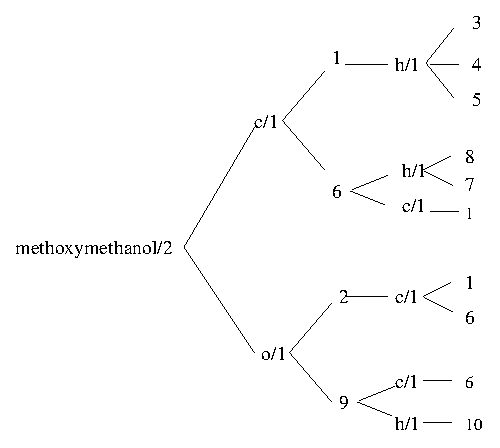
\psfig{file=figures/abstract-trie.eps}}
\caption{Methoxymethanol Represented as a Trie}\label{abstract-trie.eps}
\end{figure}
\end{example}

At a detailed level, given a fixed term traversal, an algorithm to
insert a term into a trie traverses the trie in {\em matching mode} as
long as the current component of the term matches a child of the
current node of the trie.  If the algorithm remains in matching mode
when the trie is exhausted, it reports a match.  Otherwise, if the
traversal finds a component that does not match, the algorithm begins
inserting the elements, reporting {\em no match} when the traversal
terminates.  The {\em answer check/insert} and {\em subgoal
check/insert} steps of tabling systems both require a check and an
insert if the term is not present.  This reasoning leads to a useful
result.

In the trie insertion algorithm, a simple index check is made to see
if the next element of the term exists as a child of the current node
of the trie.  Since it performs a variant check, the algorithm can
treat each unique variable as a unique constant, and is equivalent to
indexing a ground term.  Figure \ref{concrete-trie.eps} shows the trie
for Example \ref{simple-trie} as an answer trie for the call {\tt ?-
methoxymethanol(X,Y). } The links from nodes to their children are
used to traverse the trie in the check/insert operations.  The tries
also contain a link from each node to its sibling, if any.  In Version
\version\ of XSB, the insertion algorithm searches sequentially through the
list of sibling links until the list reaches a predefined size, at
which time it reconfigures the list into a hash table.  The hash
tables are then reconfigured dynamically as they fill up.  Each path in
the trie corresponds to an answer (or subgoal).  There is also a link
from each node to its parent, for loading answer clauses, as well as a
sequential list of leaf nodes, to support backtracking through answer
clauses.  

\begin{figure}[htbp]
\mbox{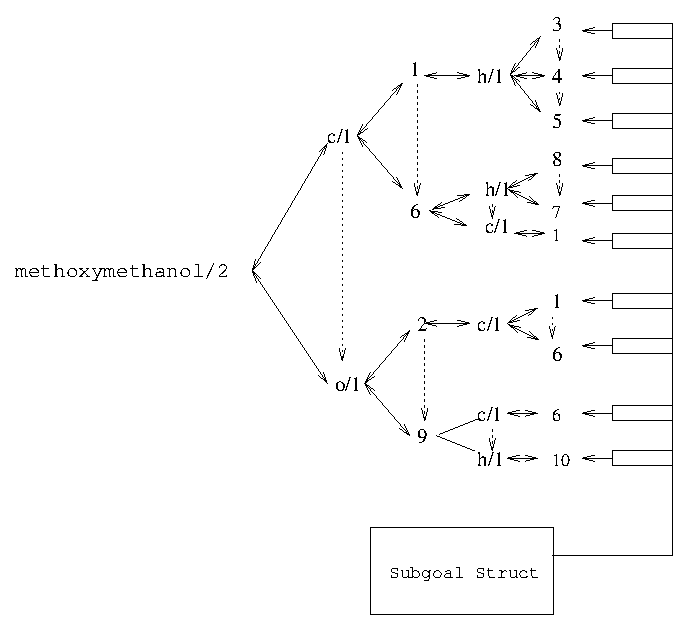
\psfig{file=figures/concrete-trie3.eps}}
\caption{Methoxymethanol as Tabled Answer Clauses}\label{concrete-trie.eps}
\end{figure}

\subsection{Substitution Factoring} \label{impl-sub-fac}

In the SLG-WAM under variant check for call, answers are always
associated with a particular subgoal.  Given a call, $A$, any answer
for $A$ must be subsumed by $A$, and can be represented as $A\theta$.
The core idea of substitution factoring is to store only the
substitution $\theta$ for each answer, and to create a mechanism for
returning answers to active subgoals that is proportional to the size
of $\theta$ rather than the size of $A$.  In the language of tabling,
substitution factoring ensures that answer tries contain no
information found in their associated subgoal tries.

Need to rewrite!

In order to explain the implementation of substitution factoring, we
consider first the creation of a (SLG-)WAM choice point for a
non-tabled program clause.  The WAM creates a choice point by copying
the program registers at the time of the call --- including registers
representing each argument of the goal.  As discussed in the previous
section, the entire tabled subgoal needs to be traversed at call time.
During the subgoal traversal, a set of free variables can be obtained.
If the subgoal is non-redundant, a generator choice point is created
which will backtrack through program clauses as explained in Section
\ref{impl-data-structs}.  However, instead of copying {\em arguments}
of the subgoal into the choice point, only the {\em free variables} of
the call are copied.  If the subgoal is redundant, program clause
resolution is not used.  Instead, an active subgoal frame is created,
which serves as an environment into which answers can be returned.
Like the generator choice points, these active subgoal frames contain
only the free variables of the subgoal.  In either case, bindings to
the dereferenced values of these variables are trailed through forward
execution, whether it is program clause or answer clause resolution.
The values are untrailed through backtracking just as argument cells
would be without substitution factoring.  When an answer to a tabled
subgoal is detected, the dereferenced values of the variable cells are
copied from the generator choice point directly into the table, and
can later be loaded directly into the active subgoal frames during
answer return.

Substitution factoring adds a slight overhead to subgoal check/insert
due to its more sophisticated handling of variables: during subgoal
traversal, pointers to the variables must be copied into the generator
choice point or the active subgoal frame.

Because the active subgoal frames and generator choice points contain
only variable cells, saving and loading of answers is proportional to
the number of free arguments of a Datalog subgoal.  But substitution
factoring is more powerful than this.  Figure
\ref{shared-trie.eps} shows a trie using substitution factoring for
the subgoals {\tt methoxymethanol(c(X),c(Y))}, and {\tt
methoxymethanol(c(X),o(Y))}.  For each answer to these calls, two
elements need to be checked or inserted rather than the four that
would need to be checked or inserted without substitution factoring.
For instance, the answer {\tt methoxymethanol(o(2),c(1))}, needs to
only check or copy the {\tt 2}, and {\tt 1}, rather than {\tt o(2)},
and {\tt c(1)}.  In fact, the cost of answer check/insert, and of
answer backtracking is proportional to the size of the {\em answer
substitution}, a simple concept whose meaning we make precise.

Clearly, the size of an answer substitution of a subgoal $S$ and
answer $A$ is less than or equal to the size of the answer $A$.  For
the program in example 1, an actual form of the subgoal for
$a_{bf}(X,Y)$ might be {\tt a(1,Y)}, while the form of an answer might
be {\tt a(1,2)}.  If so, answer substitution would be $\{Y \leftarrow
2 \}$ and substitution factoring will store only the value $2$ (and
associated pointers) rather than the pair $(1,2)$. In summary:

Perhaps too formal, but the point is probably well to make.

\begin{proposition} \rm
Let $S$ be a subgoal for which substitution factoring is used,
and $A$ a given answer.  Then both answer check/insert and
answer backtracking can be performed in cost proportional to
the size of the answer substitution of $S$ and $A$.
\end{proposition}

%%\begin{figure}[htbp]
%%\mbox{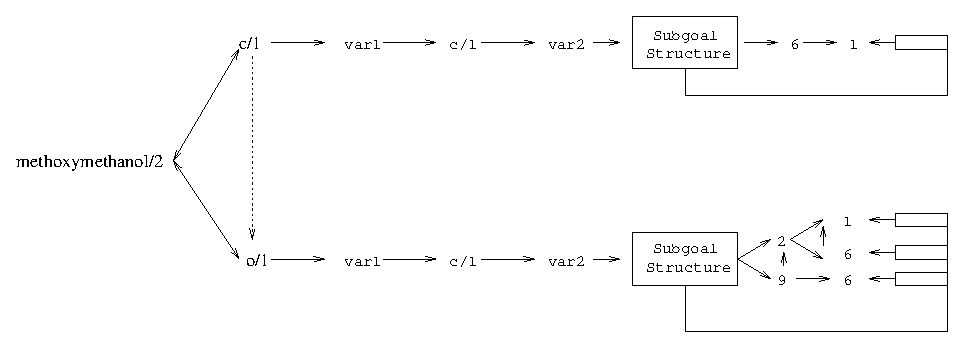
\psfig{file=figures/shared-trie4.eps}}
%%\epsfxsize=390pt
%%\epsfbox{/home/u17/sbprolog/PSB-terry/papers/figures/shared-trie4.eps}
%%\caption{Substitution Factoring for Methoxymethanol}\label{shared-trie.eps}
%%\end{figure}

This section has assumed that a variant check is used for subgoals.
Work is presently underway to determine in what manner substitution
factoring can be extended if a subsumption check is made for subgoals
instead.  As an example of one of the issues which arise here, suppose
analysis tells us that program evaluation will make a set of specific
calls, $S_I$, which are all instances of a more general call $S$.
Then we would like to determine an order of traversal for $S$ which
will minimize (under some measure) the bindings needed by each of the
$S_i$ to backtrack through the relevant answer clauses.  The process
of building the table for $S$ becomes $adaptive$ in the sense of
\cite{SRR94}, and similar optimality results may be possible.

\section*{Bibliographic Notes}

Details of XSB's implementation of tries is given in \cite{RRSSW94}.

Shorten this if we actually want to include it.

Substitution factoring bears a certain resemblance to the factoring of
\cite{NRSU89} (here termed NRSU factoring) in that both reduce the
number of arguments copied into or out of a table.  However, since
substitution factoring is dynamic rather than static, as is NRSU, it
has different characteristics.  Whether a predicate is NRSU factorable
is undecidable so that substitution factoring may reduce arguments not
reduced by NRSU factoring.  Further, substitution factoring is defined
for non-Datalog programs.  On the other hand \cite{NRSU89} introduces
additional optimizations based on the factored program.  These
optimizations can transform certain right and double recursions into
left recursions, an important transformation not done by substitution
factoring.

***********************************************************************
Below: Break out DNF example if we indeed want to keep it.

Refer back to table tries.

Put simply, unification factoring factors out bindings common to
clause heads of a predicate, transforming a program into a trie-like
structure through which backtracking can be efficiently performed.
Example \ref{impl-uni-fac} illustrates the effect of unification
factoring on a simple program fragment.  Formally, unification
factoring is not an indexing technique, but rather a transformation
that minimizes the maximal cost of backtracking through a set of
clause heads using SLD resolution, a cost which occurs when the call
is completely uninstantiated.  Even so, unification factoring can
provide a significant speedup for a variety of programs partly by
providing better indexing of clause heads.  As examples, for the
well-known Dutch National Flag example
\cite{StSh86} a speedup of 200\% is observed due primarily to indexing,
while retrievals from a chemical database are sped up by an average of
about 300\% due to a mixture of indexing and improved backtracking.
Since each of the auxiliary predicates of the transformed program (in
Example \ref{impl-uni-fac} {\tt p\_f/2} and {\tt p\_gf/2}) are indexed
as in Prolog, speedup from indexing occurs when common arguments or
functor positions are factored out and the indexing of auxiliary
predicates can be used to advantage.

\begin{example} \rm \label{impl-uni-fac}
The program clauses
\begin{verbatim}
  p(g(a),f(X)).        
  p(g(b),f(1)).       
  p(g(a),f(a)).       
  p(g(X),Y).   
\end{verbatim}
Are transformed into the clauses
\begin{verbatim}
   p(g(X),Y):- p_g(X,Z)
   p(g(X),Y).

   p_g(X,f(Y)):- p_gf(X,Y).
   p_g(X,Y).

   p_gf(a,Z).
   p_gf(a,a).
   p_gf(b,1).
\end{verbatim}
representing the the trie-like structure
\ \\
\begin{center}
\mbox{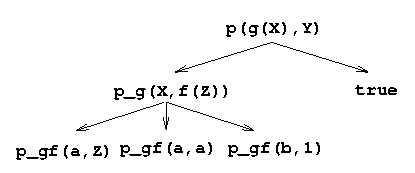
\psfig{file=figures/trans-ind.eps}}
\end{center}
\ \\
Note that the call {\tt p(X,Y)} will perform 4 bindings and 4
unbindings of variable addresses in the transformed program, while the
same call would perform 12 bindings and 12 unbindings in the original
program.
\end{example}

Unification factoring can be implemented as a program transformation
and as such provides speedups for most Prolog systems: improvements
for Quintus and SICTUS have been observed as well as for XSB.  Some
minor compiler changes are needed to produce the 200\% - 300\%
speedups mentioned above.  As shown in Example
\ref{impl-uni-fac-hack}, it is useful for a system to have the
ability to index on the outer functor of a given argument, not just
the first argument.  Also, to avoid register movement in the WAM, it
is useful to be able to treat arguments which have been factored out
as void variables.  Finally, calls to intermediate predicates may use
jumps rather than the WAM {\tt execute} instruction, since they do
not need to be traced, to handle interrupts, or permit redefinition.

\begin{example} \rm \label{impl-uni-fac-hack}
The predicate
\begin{verbatim}
   p(a,b,X).
   p(a,c,Y)
\end{verbatim}
is more efficiently transformed into 
\begin{verbatim}
   p(a,X,Y):- p_a(void,X,Y).

   :- index(p_a/3,2).
   p_a(_,b,W).
   p_a(_,c,W).
\end{verbatim}
treating the factored argument as void and indexing on the
second argument, than into
\begin{verbatim}
   p(a,X,Y):- p_a(X,Y).

   p_a(b,W).
   p_a(c,W).
\end{verbatim}
\end{example}
since the latter fragment requires register movement
instructions to move the second argument into the first and the
third into the second.

If modes are known, a transformation like unification factoring can be
used to index instantiated input arguments as well as to improve the
backtracking of uninstantiated arguments.  Given knowledge about
modes, the complexity of obtaining transformed programs is
NP-complete.  Another question that remains open is how to extend
unification factoring to predicates which are to use SLG resolution.
Unfortunately the minimality properties of \cite{DRRSSSW94} do not
carry over to SLG resolution in a straightforward manner as can be
seen from example
\ref{impl-slg-uni-fac}.  Nevertheless, unification factoring, can
greatly improve the execution time of many programs since, in addition
to improving indexing and reducing the cost of backtracking through
clauses, it can factor out bindings from the heads of clauses so that
they do not need to be stored as answer tries.

\begin{example} \rm \label{impl-slg-uni-fac}
Let clause heads for a tabled predicate {\tt p/2} consist of 
\begin{verbatim}
   p(a,1,X):- body1.
   p(a,2,X):- body2.
   p(b,1,X):- body3.
   p(b,2,X):- body4.
\end{verbatim}
the transformed program would be
\begin{verbatim}
   p(a,X,Y):- p_a(X,Y).
   p(b,X,Y):- p_b(X,Y).

   p_a(1,X):- body1.
   p_a(2,X):- body2.
   p_b(1,X):- body3.
   p_b(2,X):- body4.
\end{verbatim}
The decision where to table the transformed program remains.  If the
last argument were uninstantiated on call, tabling {\tt p\_a/2} and
{\tt p\_b/2} would be superior under most cost criteria.  However if
the last argument were instantiated with unbounded size, the cost of
examining the call twice could make execution of the program tabled at
{\tt p\_a/2} and {\tt p\_b/2} cost arbitrarily more than the program
tabled at {\tt p/2}.  This problem is addressed in \cite{DRRS94}.
\end{example}

\section{Indexing Dynamic Program Clauses}

Something like, what is dynamic code but tables?

Traditional Prolog indexing examines only the outer functor of an {\em
index argument} of a clause head, usually the first argument.  This
strategy usually works well for most programming applications but is
clearly inadequate for database applications, which may require
separate distinct indexes (e.g. on argument 1 {\em or} argument 2) or
on multiple positions within the arguments of a clause head (as
required in example \ref{simple-trie}).

***************************************


The answer has been added to the table.  And the answer has been
returned to the suspended machine state, updating it and adding it to
the top of the stack to be continued.  Now \verb|ans(bill)| is an
answer to the entire query, so it is printed out by the top-loop, and
then the new state on the top of the stack,
\verb|ans1(Ya) :- owes(andy,Intb),avoids(Intb,Ya)|
is chosen for execution.

The next call, \verb|owes(andy,Intb)|, is made and matches a single
fact, so the configuration is updated to:
\begin{verbatim}
  tab: 1. call: avoids(andy,Ya)
           ans: ans1(bill)
          susp: ans(Ya) :- avoids(andy,Ya).

stack:
  ans1(Ya) :- avoids(bill,Ya).
\end{verbatim}

Now extending this state involves another call to the tabled
predicate.  This call is not already in the table, so we add it and
move to the configuration:
\begin{verbatim}
  tab: 1. call: avoids(andy,Ya)
           ans: ans1(bill)
          susp: ans(Ya) :- avoids(andy,Ya).
       2. call: avoids(bill,Ya)
          susp: ans1(Ya) :- avoids(bill,Ya).

stack:
  ans2(Yc) :- owes(bill,Yc).
  ans2(Yc) :- owes(bill,Intc),avoids(Intc,Yc).
\end{verbatim}
Continuing by taking the top state from the stack, we get to:
\begin{verbatim}
  tab: 1. call: avoids(andy,Ya)
           ans: ans1(bill)
          susp: ans(Ya) :- avoids(andy,Ya).
       2. call: avoids(bill,Ya)
          susp: ans1(Ya) :- avoids(bill,Ya).

stack:
  ans2(carl) :- .
  ans2(Yc) :- owes(bill,Intc),avoids(Intc,Yc).
\end{verbatim}
This gives us a new answer to a call, so we add it to the table and
schedule the suspended machine:
\begin{verbatim}
  tab: 1. call: avoids(andy,Ya)
           ans: ans1(bill)
          susp: ans(Ya) :- avoids(andy,Ya).
       2. call: avoids(bill,Ya)
           ans: ans2(carl)
          susp: ans1(Ya) :- avoids(bill,Ya).

stack:
  ans1(carl) :- .
  ans2(Yc) :- owes(bill,Intc),avoids(Intc,Yc).
\end{verbatim}
This gives us a new answer to the first call, so we add it to the
table and schedule the suspended machine:
\begin{verbatim}
  tab: 1. call: avoids(andy,Ya)
           ans: ans1(bill), ans1(carl)
          susp: ans(Ya) :- avoids(andy,Ya).
       2. call: avoids(bill,Ya)
           ans: ans2(carl)
          susp: ans1(Ya) :- avoids(bill,Ya).

stack:
  ans(carl) :- .
  ans2(Yc) :- owes(bill,Intc),avoids(Intc,Yc).
\end{verbatim}
Here we have an answer for the initial goal, so it is printed out for
the user, and execution proceeds (assuming the user entered a
\verb|;|) with the new top-of-stack state.  Here the call to 
\verb|owes(bill,Intc)| matches a fact and we update the configuration
to:
\begin{verbatim}
  tab: 1. call: avoids(andy,Ya)
           ans: ans1(bill), ans1(carl)
          susp: ans(Ya) :- avoids(andy,Ya).
       2. call: avoids(bill,Ya)
           ans: ans2(carl)
          susp: ans1(Ya) :- avoids(bill,Ya).

stack:
  ans2(Yc) :- avoids(carl,Yc).
\end{verbatim}
Extending this state involves another new call to a tabled predicate,
so we add it to the table and get:
\begin{verbatim}
  tab: 1. call: avoids(andy,Ya)
           ans: ans1(bill), ans1(carl)
          susp: ans(Ya) :- avoids(andy,Ya).
       2. call: avoids(bill,Ya)
           ans: ans2(carl)
          susp: ans1(Ya) :- avoids(bill,Ya).
       3. call: avoids(carl,Yc)
          susp: ans2(Yc) :- avoids(carl,Yc).

stack:
  ans3(Yd) :- owes(carl,Yd).
  ans3(Yd) :- owes(carl,Intd),avoids(Intd,Yd).
\end{verbatim}
Matching \verb|owes(carl,Yd)| yields a new answer, \verb|ans3(bill)|,
for the table, so it is added and the suspended state scheduled:
\begin{verbatim}
  tab: 1. call: avoids(andy,Ya)
           ans: ans1(bill), ans1(carl)
          susp: ans(Ya) :- avoids(andy,Ya).
       2. call: avoids(bill,Ya)
           ans: ans2(carl)
          susp: ans1(Ya) :- avoids(bill,Ya).
       3. call: avoids(carl,Yc)
           ans: ans3(bill)
          susp: ans2(Yc) :- avoids(carl,Yc).

stack:
  ans2(bill) :- .
  ans3(Yd) :- owes(carl,Intd),avoids(Intd,Yd).
\end{verbatim}
So now we have a new answer for table entry 2, so it is added, and its
suspended machine is scheduled:
\begin{verbatim}
  tab: 1. call: avoids(andy,Ya)
           ans: ans1(bill), ans1(carl)
          susp: ans(Ya) :- avoids(andy,Ya).
       2. call: avoids(bill,Ya)
           ans: ans2(carl), ans2(bill)
          susp: ans1(Ya) :- avoids(bill,Ya).
       3. call: avoids(carl,Yc)
           ans: ans3(bill)
          susp: ans2(Yc) :- avoids(carl,Yc).

stack:
  ans1(bill) :- .
  ans3(Yd) :- owes(carl,Intd),avoids(Intd,Yd).
\end{verbatim}
Now we have an answer for table entry 1, but it is a duplicate answer;
we already have the answer \verb|bill| for that call.  So we do {\em not}
add it again to the table, but simply fail.  Thus we extend the next
state on the stack, which results in a match of
\verb|owes(carl,Intd)|, which leads to the configuration:
\begin{verbatim}
  tab: 1. call: avoids(andy,Ya)
           ans: ans1(bill), ans1(carl)
          susp: ans(Ya) :- avoids(andy,Ya).
       2. call: avoids(bill,Ya)
           ans: ans2(carl), ans2(bill)
          susp: ans1(Ya) :- avoids(bill,Ya).
       3. call: avoids(carl,Yc)
           ans: ans3(bill)
          susp: ans2(Yc) :- avoids(carl,Yc).

stack:
  ans3(Yd) :- avoids(bill,Yd).
\end{verbatim}
In extending this state, we look up the call \verb|avoids(bill,Yd)| in
the table and find that it is already there.  (We check for a variant
of the call, i.e. a call that differs only in the names of its
variables.)  So we add the machine state to those suspended on that
table entry, and schedule new computations for the answers currently
in the table, obtaining:
\begin{verbatim}
  tab: 1. call: avoids(andy,Ya)
           ans: ans1(bill), ans1(carl)
          susp: ans(Ya) :- avoids(andy,Ya).
       2. call: avoids(bill,Ya)
           ans: ans2(carl), ans2(bill)
          susp: ans1(Ya) :- avoids(bill,Ya).
                ans3(Yd) :- avoids(bill,Yd).
       3. call: avoids(carl,Yc)
           ans: ans3(bill)
          susp: ans2(Yc) :- avoids(carl,Yc).

stack:
  ans3(carl) :- .
  ans3(bill) :- .
\end{verbatim}
Now the top state on the stack is a new answer for table entry 3, so
it is added, and the suspended state is schedule with this new answer:
\begin{verbatim}
  tab: 1. call: avoids(andy,Ya)
           ans: ans1(bill), ans1(carl)
          susp: ans(Ya) :- avoids(andy,Ya).
       2. call: avoids(bill,Ya)
           ans: ans2(carl), ans2(bill)
          susp: ans1(Ya) :- avoids(bill,Ya).
                ans3(Yd) :- avoids(bill,Yd).
       3. call: avoids(carl,Yc)
           ans: ans3(bill), ans3(carl)
          susp: ans2(Yc) :- avoids(carl,Yc).

stack:
  ans2(carl) :- .
  ans3(bill) :- .
\end{verbatim}
Now the top state is an answer for table entry 2, but it is a
duplicate answer, so the machine is failed, and simply deleted,
yielding the configuration:
\begin{verbatim}
  tab: 1. call: avoids(andy,Ya)
           ans: ans1(bill), ans1(carl)
          susp: ans(Ya) :- avoids(andy,Ya).
       2. call: avoids(bill,Ya)
           ans: ans2(carl), ans2(bill)
          susp: ans1(Ya) :- avoids(bill,Ya).
                ans3(Yd) :- avoids(bill,Yd).
       3. call: avoids(carl,Yc)
           ans: ans3(bill), ans3(carl)
          susp: ans2(Yc) :- avoids(carl,Yc).

stack:
  ans3(bill) :- .
\end{verbatim}
This answer for table entry 3 is also a duplicate, so the machine
state is deleted.  Now the scheduling stack is empty and the
computation terminates, having produced all and only the correct
answers to the initial query.
